
\begin{multicols}{2}
On considère le pavé droit $ABCDEFGH$ tel que $DE=DC=3$~cm, $DA=4$~cm et $DB=5$~cm.
\begin{enumerate}
	\item 
\begin{enumerate}
\item Sur la figure, représenter, en vert, la section de ce pavé par
  le plan passant par $B$ et $D$ et parallèle à l'arête $(CH)$.
	\item Dessiner en vraie grandeur cette section sur votre
          copie. On indiquera clairement les dimensions de celle-ci.
\end{enumerate}
	\item 
\begin{enumerate}
	\item Représenter sur la figure en rouge la section de ce pavé
          par le plan passant par $I$ et parallèle à la face $ABGF$.
	\item Dessiner en vraie grandeur cette section sur votre
          copie. On indiquera clairement les dimensions de celle-ci.
\end{enumerate}
\end{enumerate}
\begin{center}
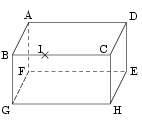
\includegraphics[scale=1]{RepS-41.png} 
\end{center}
\end{multicols}

